\documentclass[article,type=msc,colorback,accentcolor=tud7b]{tudthesis}

%TODO: Markus Zopf

\usepackage[english]{babel}
\usepackage{amsmath}
\usepackage{array}
\usepackage{enumitem}
\usepackage{listings}
\usepackage{floatrow}
\usepackage{multirow}
\usepackage{subfig}
% Table float box with bottom caption, box width adjusted to content
\newfloatcommand{capbtabbox}{table}[][\FBwidth]
\restylefloat{table}
\newcolumntype{C}[1]{>{\centering\let\newline\\\arraybackslash\hspace{0pt}}m{#1}}

\usepackage[
    backend=biber, % biber ist das Standard-Backend für Biblatex. Für die Abwärtskompatibilität kann hier auch bibtex oder bibtex8 gewählt werden (siehe biblatex-Dokumentation)
    style=alphabetic, %numeric, authortitle, alphabetic etc.
    autocite=plain, % Stil, der mit \autocite verwendet wird
    sorting=nty, % Sortierung: nty = name title year, nyt = name year title u.a.
    sortcase=false,
    url=false,
    hyperref=auto,
]{biblatex}

\addbibresource{bibliography.bib}

\newcommand{\getmydate}{%
  \ifcase\month%
    \or Januar\or Februar\or M\"arz%
    \or April\or Mai\or Juni\or Juli%
    \or August\or September\or Oktober%
    \or November\or Dezember%
  \fi\ \number\year%
}

\begin{document}
  \thesistitle{Sentiment classification of chess annotations}{}
  \author{Florian Beck}
  \referee{Prof. Dr. Johannes Fürnkranz}{}
  \department{Fachbereich Informatik}
  \group{Knowledge Engineering Group}
  \dateofexam{\today}{\today}
  %\tuprints{12345}{1234}
  \makethesistitle
  \affidavit{Florian Beck}
  
  \input{abstract}
  %TODO: auch in deutsch
  \clearpage
  
  \setcounter{tocdepth}{3}
  \tableofcontents
  \setcounter{page}{3}
  \clearpage
  
  \listoffigures
  \listoftables
  \clearpage
  
  \section{Introduction}

  \subsection{Motivation}

  \subsection{Problem description}

  \subsection{Goal of the thesis}
    - is it possible to "convert" a chess annotation comment to the appropiate symbol by using a classifier

  \subsection{Structure of the thesis}
  \clearpage
  
  \section{Basics (TODO)}
    Sentiment Analysis and classification, Ordinal Classification, Word Embeddings, TF-IDF
    mindestens 5 Seiten
  
  \subsection{Multiclass classification}
  \label{subsec:multiclass_classification}
  
    \begin{figure}[H]
      \centering
      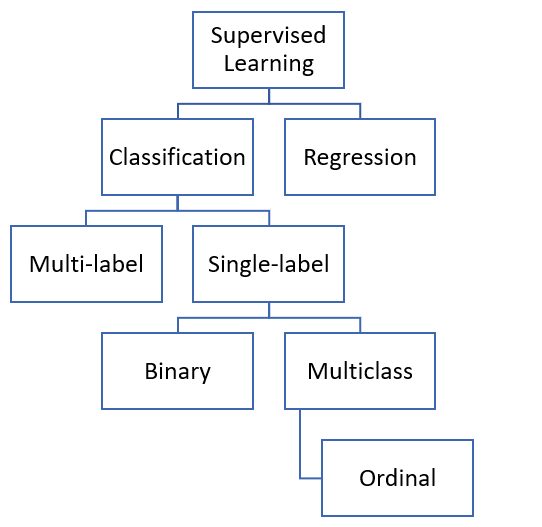
\includegraphics{images/problem_hierarchy_supervised_learning}
      \caption{Problem hierarchy of supervised learning}
      \label{fig:problem_hierarchy_supervised_learning}
    \end{figure}

    \begin{figure}[H]
      \centering
      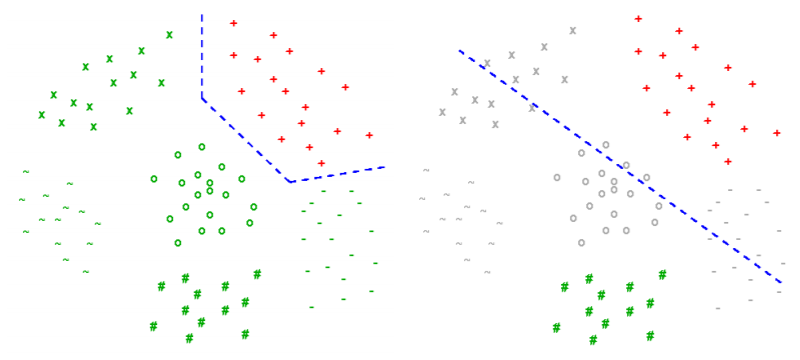
\includegraphics{images/one_against_all_or_one}
      \caption[One-against-all vs. one-against-one approach]{One-against-all (left) vs. one-against-one approach (right)\protect\footnotemark}
      \label{fig:one_against_all_or_one}
    \end{figure}
    
    \footnotetext{J. Fürnkranz, Machine Learning and Data Mining | Learning Rule Sets, V3.0, p.45\&47}
  
    \begin{table}[H]
      \centering
      \setlength\tabcolsep{1.5pt}
      \subfloat[One-against-all]{
      \begin{tabular}{ |C{1.5cm}|C{0.5cm}|C{0.5cm}|C{0.5cm}|C{0.5cm}|C{0.5cm}| } 
        \hline
        class & $f_{1}$ & $f_{2}$ & $f_{3}$ & $f_{4}$ & $f_{5}$ \\ \hline
        1 & 1 & 0 & 0 & 0 & 0 \\ \hline
        2 & 0 & 1 & 0 & 0 & 0 \\ \hline
        3 & 0 & 0 & 1 & 0 & 0 \\ \hline
        4 & 0 & 0 & 0 & 1 & 0 \\ \hline
        5 & 0 & 0 & 0 & 0 & 1 \\ \hline
      \end{tabular}
      }
      \quad
      \subfloat[One-against-one]{
      \begin{tabular}{ |C{1.5cm}|C{0.5cm}|C{0.5cm}|C{0.5cm}|C{0.5cm}|C{0.5cm}|C{0.5cm}|C{0.5cm}|C{0.5cm}|C{0.5cm}|C{0.5cm}| } 
        \hline
        class & $f_{1}$ & $f_{2}$ & $f_{3}$ & $f_{4}$ & $f_{5}$ & $f_{6}$ & $f_{7}$ & $f_{8}$ & $f_{9}$ & $f_{10}$ \\ \hline
        1 & 1 & 1 & 1 & 1 & 0 & 0 & 0 & 0 & 0 & 0 \\ \hline
        2 & 1 & 0 & 0 & 0 & 1 & 1 & 1 & 0 & 0 & 0 \\ \hline
        3 & 0 & 1 & 0 & 0 & 1 & 0 & 0 & 1 & 1 & 0 \\ \hline
        4 & 0 & 0 & 1 & 0 & 0 & 1 & 0 & 1 & 0 & 1 \\ \hline
        5 & 0 & 0 & 0 & 1 & 0 & 0 & 1 & 0 & 1 & 1 \\ \hline
      \end{tabular}
      }
      
      \subfloat[Exhaustive error-correcting output code]{
      \begin{tabular}{ |C{1.5cm}|C{0.5cm}|C{0.5cm}|C{0.5cm}|C{0.5cm}|C{0.5cm}|C{0.5cm}|C{0.5cm}|C{0.5cm}|C{0.5cm}|C{0.5cm}|C{0.5cm}|C{0.5cm}|C{0.5cm}|C{0.5cm}|C{0.5cm}| } 
        \hline
        class & $f_{1}$ & $f_{2}$ & $f_{3}$ & $f_{4}$ & $f_{5}$ & $f_{6}$ & $f_{7}$ & $f_{8}$ & $f_{9}$ & $f_{10}$ & $f_{11}$ & $f_{12}$ & $f_{13}$ & $f_{14}$ & $f_{15}$ \\ \hline
        1 & 0 & 0 & 0 & 0 & 0 & 0 & 0 & 0 & 0 & 0 & 0 & 0 & 0 & 0 & 0 \\ \hline
        2 & 0 & 0 & 0 & 0 & 0 & 0 & 0 & 1 & 1 & 1 & 1 & 1 & 1 & 1 & 1 \\ \hline
        3 & 0 & 0 & 0 & 1 & 1 & 1 & 1 & 0 & 0 & 0 & 0 & 1 & 1 & 1 & 1 \\ \hline
        4 & 0 & 1 & 1 & 0 & 0 & 1 & 1 & 0 & 0 & 1 & 1 & 0 & 0 & 1 & 1 \\ \hline
        5 & 1 & 0 & 1 & 0 & 1 & 0 & 1 & 0 & 1 & 0 & 1 & 0 & 1 & 0 & 1 \\ \hline
      \end{tabular}
      }
      \caption[Output codes for a multiclass classification problem]{Different output codes for a multiclass classification problem with five classes}
      \label{tab:exhaustive_ecoc}
    \end{table}

    \begin{figure}[H]
      \centering
      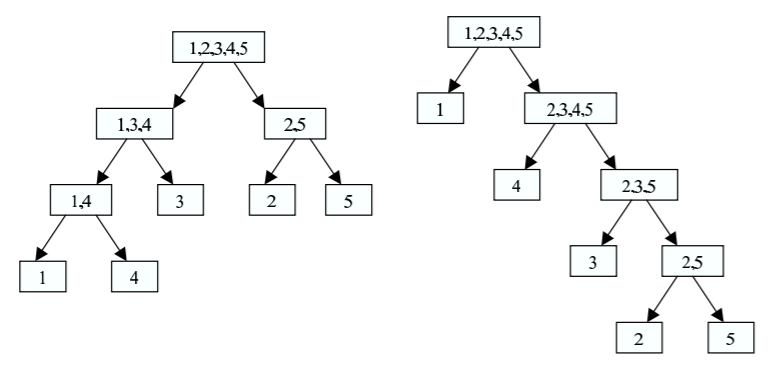
\includegraphics{images/nested_dichotomies}
      \caption[Two nested dichotomies]{Two nested dichotomies for a multiclass problem with five classes \autocite{Dong2005}\protect\footnotemark}
      \label{fig:nested_dichotomies}
    \end{figure}

  \subsection{Ordinal classification}
  \label{subsec:ordinal_classification}
  
  \subsection{Cost-sensitive learning}
  \label{subsec:cost_sensitive_learning}

  \subsection{Word embeddings}
  \label{subsec:word_embeddings}
  \clearpage
  
  \section{Concept}
  
    This chapter describes how to solve a general problem of extracting knowledge out of natural language sources and defines which steps have to be considered. Therefore, in the following the focus is set on universal approaches to accomplish such a task. Specific ideas and solutions adjusted to the sentiment classification task for chess annotations will be dealt with in section~\ref{sec:experimental_setup}. \\\\
    The solution of a text mining problem comprises several steps from definition to evaluation. Figure~\ref{fig:text_mining_pipeline} shows a possible process model based on approaches of \citeauthor{Schieber2014} \autocite{Schieber2014} and \citeauthor{Kwartler2017} \autocite{Kwartler2017}. The model consists of six steps, which are now presented one after the other.
    
    \begin{figure}[H]
      \centering
      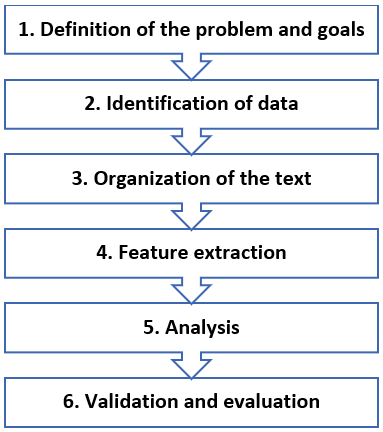
\includegraphics{images/text_mining_pipeline}
      \caption{Processing pipeline of text mining}
      \label{fig:text_mining_pipeline}
    \end{figure}
  
  \subsection{Definition of the problem and goals}
  \label{subsec:definition_of_the_problem_and_goals}
    In the first step we have to define the problem we want to solve. According to \citeauthor{Mitchell1997} a learning problem generally reads as follows: Improve over task $T$, with respect to performance measure $P$, based on experience $E$. The goal is therefore to generalize the experience in a way that allows to improve your performance on the task \autocite[Chapter~1]{Mitchell1997}.
    \begin{itemize}
      \item Task $T$
      
        The task can be formulated by a simple verbal description, e.g. “play the game Connect Four” or “sort the e-mail into the categories spam and no-spam”. A more formally approach requires the exact definition of the input and the output of the task. \\
        The input could be a set of attribute-value pairs, e.g. in relational data, where each input would have the same set of attributes. But since there is no restriction to the input data to be homogeneous the input can be plain text as well. A possible input of natural language could be represented by a whole book, by a (web) page, by a paragraph or just by one sentence. In certain cases, even a single letter is an appropriate input, e.g. for the detection of handwritten letters. \\
        As well as for the input we need to determine the type of output we want to receive. But not only the type, also the precision in the range of values is important for the difficulty of the task. In the case of product reviews the easiest output “good review vs. bad review” could be complicated by using the ten values of a five-star rating or by distinguishing between different ratings for the quality, the price-performance ratio, the delivery etc. The aforementioned examples have in common that the number of possible output values is fixed which means a classification problem is concerned, not a regression problem. In the following the focus will be set on classification tasks.
      \item Performance measure $P$
      
        The straightforward approach for classification tasks would be to count the instances with the correct output and divide this number by the total number of instances. This value is called accuracy. Just as well the complementary probability for misclassified instances, called error rate, can be observed. However, there are also possibilities to weight the classifications. If there are instances that are more important than others these instances can be multiplied or associated with a weight greater than one. Furthermore, the misclassifications can be considered separately dependent on the correct and predicted class. In spam classification, it is usually significantly worse to classify a no-spam e-mail as spam than the other way around. To map this idea, we can assign to each pair of correct and predicted class a weight value. \\
        This type of measurement is not appropriate for regression tasks. Dependent on the exactitude of the values the probability that the predicted value is exact the correct one is low. Instead of demanding an exact prediction, we can also use the difference between correct and predicted value as the performance (MAE) or the squared difference (MSE) \autocite[Chapter~5.8]{Witten2005}. \\
        In the case of an unsupervised problem only subjective estimates can be used. The learned model and its output are evaluated by an expert, which might entail a high expenditure of time and money. \\
        The validation and evaluation techniques will be dealt with in detail in subsection~\ref{subsec:validation_and_evaluation}.
      \item Experience $E$
      
        The experience of a learning problem is the knowledge the learner already possesses before solving the task. For example, a student solves exercises to gain experience before writing an exam. In machine learning, the experience is achieved through the acquisition of knowledge from databases. In both cases the learner tries to improve the performance in the task by the usage of the knowledge of similar data. If no similar data is already known, the learner can just guess the correct output. For this reason, a sufficiently large amount of data should be available to the learner in order to increase the experience and therefore also the chance to solve the task in the desired manner.
    \end{itemize}
    The following describes the procedure as generally as possible; we only assume that we face a classification problem in the field of text mining. Furthermore, the output value should be known for all instances, such that tasks of supervised learning can be applied automatically. As the input we use a document $d\in\mathbb{X}$, where $\mathbb{X}$ is the document space; and as the output a fixed set of classes $\mathbb{C}=\left\{c_{1},c_{2},\dots,c_{J}\right\}$. Using a learning method or learning algorithm, we then wish to learn a classifier or classification function $\gamma$ that maps documents to classes, i.e. $\gamma:\mathbb{X}\rightarrow\mathbb{C}$ \autocite[Chapter~13.1]{Manning2008}.
  
  \subsection{Identification of data}
    In the second step we need to find one or several data sources that offer an adequate number of instances, i.e. data sets of the previously defined input and output type. There are four characteristics to be aware of:
    \begin{itemize}
      \item Completeness
      
        Each instance of the data should be complete, i.e. we know the input and the output of the instance. All attributes of the input should be filled with a value. If they are not filled, a default value can be used or another way how to manage missing values needs to be defined. Of course, there is also a need of the completeness of the output value. Otherwise, the instance can not be used for training nor for the evaluation.
      \item Format
      
        In addition to the completeness, the data needs to be in the same format. Using data from data sources with different syntactical structure requires a pre-processing, such that the data can be compared and processed in a similar way in further steps. This involves the order and the atomicity or distribution of the data.
      \item Quantity
      
        To be able to discover meaningful knowledge, we need a minimal data volume, usually starting from several hundreds or thousands of instances. This concerns also the absolute and the relative amount for each class or even for the most important attribute values. An upper limit of instances does not exist. However, sufficient computing and storage capacities must be available.
      \item Quality
      
        The quality of the data goes along with the completeness, but it goes one step further. The desired values should not only be existent but also accomplish quality requirements, such as observing minimal and maximal values (numeric attributes) or lengths (linguistic attributes), providing a minimal precision or being available in a specific language. Analogous to checks and other constraints in databases, the data could be validated before using it in the mining process.
    \end{itemize}
    After completing the second step we end up with an appropriate data set for the task defined in the first step. The data is in a homogeneous representation, but not necessarily in a structured form.

  \subsection{Organization of the text}
    A big part of all data in the internet exists in the form of natural language. Usually, it is hard to evaluate the information contained in this data, because it is not structured in the same way. For example, in product reviews every customer can write his comment in a different kind, so that there is neither a certain order of the information nor a specification, which information the comment should provide. However, on the basis of an additional star rating it is possible to get a fast assessment of the customer’s attitude towards the product. So, if there is a need of further evaluation, it is helpful to have the data in a structured form instead of an unstructured form. \\\\
    Often it is not desirable or even impossible to get the unstructured data directly in a structured form, so we have to do the transformation on our own. This process of converting the data from an unstructured into a structured form is called information extraction. It is assumed that the input data is a single string, i.e. a sequence of characters. The sequence can contain just a few characters (e.g. tweets, comments) or thousands of characters (e.g. book contents). Even if in the most common cases this string is natural language, the procedure is similar for other input strings as well. In order not to falsify the data, we have to take into account the character encoding. The goal of this step is to reorganize the input from a string to a collection of tokens, also known as lexing or tokenization. This process takes place in three sub-steps:
    \begin{itemize}
      \item Token identification
      
        A lexical token, shortly token, is a string with an identified meaning. The input string is split into substrings where each substring without meaning is discarded and all others are stored as tokens. The definition of a token depends on the use case. In natural language processing, the standard approach is to use blanks or other whitespace characters and interpunctuation symbols as separators of tokens. As a result, there are words as tokens. This general solution can be customized by interpreting whitespace characters and interpunctuation symbols (or combinations of them) as tokens. Words can also be further split at a hyphen or split into characters. The other way around, two or more words can be combined to one token, e.g. for names of persons or places (“New York”) or for usual phrases (“and so on”). All of the parts of the string that do not contain any information should be removed directly. Frequently used words as “and” or “that”, also called stopwords, do not provide added value and can be removed from the token collection. There are lists of stopwords available for common textual resources, but they may be customized for specific data sets. Other challenges in natural language processing include handling spelling mistakes, acronyms and special characters such as smileys \autocite{Kharde2016}.
      \item Normalization
      
        In this step we want to find tokens that should be treated as identical, even if the strings of the token are different. In the simplest case we can make the interpretation of a token case-insensitive by converting all occurrences into lowercase. Before doing so it should be ensured that no information is lost as a result. In sentiment analysis, a large proportion of uppercase letters could indicate rage. Other types of normalization are lemmatization and stemming. Words in natural language can be modified by inflection, most of all by conjugation (modification of verbs caused by person, tense etc.) and declination (other part of speech caused by case, gender, number etc.). Lemmatization brings all parts of speech back into its basic form, e.g. the singular nominative case for nouns or the infinitive for verbs. Stemming reduces all words independent of its part of speech to the word stem, which need not be a proper word. Though, as a consequence information about the original token get lost which can lead to incompatibilities with the further analysis in the next steps. Obviously, the order of normalization and token merging or deletion from the first step may influence the result as well and should therefore be made consciously. Besides, not only the input, but also the output can be normalized. The merging of two or more output values to one joint class can also be considered as a normalization step.
      \item Categorization
      
        This step deals with the syntactic and the semantic analysis of the tokens. Syntactic analysis, also known as parsing, is the process of assigning each token a category describing its function in the context. In classical parsing of code files, categories can be identifiers, keywords, literals etc., in parsing of natural language resources, categories can be nouns, verbs, adjectives etc. Last-mentioned is known as part-of-speech-tagging (POS-tagging). Building on the syntactic analysis we can also assign a meaning to the token in addition to the category. This process is called semantic analysis and can cover difficulties of synonyms and polysemes (ambiguous words). These semantical relations and more for English vocabulary are provided by the lexical database WordNet\footnote{\url{https://wordnet.princeton.edu/}}.
    \end{itemize}
    After finishing the chosen approaches of those three steps, we obtain the unstructured text data in a structured collection of tokens, possibly extended or replaced by their category or meaning. By splitting the string into tokens in the beginning, the tokens in the collection will be sorted in the same order as they occur in the input. The collection is in list form and the order is maintained. If the order and the count of tokens is irrelevant for further evaluation, a set can be used instead of a list. However, in most cases just the order is irrelevant but not the count of tokens, such that a multiset is the suitable form of collection. This multiset is known as “bag of words”.
  
  \subsection{Feature extraction}
    Based on the created output from step three, now the characteristics of the input data are to be figured out by feature extraction. The idea is to calculate various scores, such that we can compare the input data instances with each other, especially concerning the sentiment and polarity. At the end of this step we want to obtain a representation that can be passed as a training set to learning algorithms. \\\\
    The default feature extraction approach is typically used in web search engines during the indexing step in information retrieval. The input is a list of documents in bag of words-representation or something similar. This results in a document-term-matrix, where each row describes a document and each column the count of a specific term. This concept can be generalized and transferred to our question. The column remains the description of the document as a vector whereas each column is the value of a specific feature. The model is called Vector Space Model (VSM) as it represents each document as a vector of features which simplifies the comparison of two documents by cosine similarity. Possible features with direct relation to the token are:
    \begin{itemize}
      \item binary indication
      
        This feature holds the value 0, if the token does not occur, and the value 1 otherwise. This value follows immediately if the collection is represented as a simple set.
      \item term frequency (TF)
      
        This feature holds the count of the token as described in the information retrieval example. This value follows immediately if the collection is represented as a multiset. The value can be normalized by dividing it by the total number of tokens in the document. Another option is to relativize very high term frequency values by using the logarithm function.
      \item term frequency – inverse document frequency (TF-IDF)
      
        In contrast to the term frequency, TF-IDF decreases the weight by taking into account the number of documents in which a token appears. The idea is to reward rarely occurring tokens with a high feature value. If the token appears in all documents, the value will be 0. If the token appears in just one document, the value is maximal.
    \end{itemize}
    Features need not be dependent of only one token. There are more advanced features that use accumulation of several tokens like the average token length. The above-mentioned values can also all be calculated if the tokens are grouped by category \autocite{Wang2010}. For problems concerning long input texts in natural languages like author detection another appropriate feature is the lexical diversity. It calculates the ratio between the count of distinct words (vocabulary) and the total word count. \\\\
    If the collection is passed in list representation, we can additionally create features by using combinations of sequential tokens. These sequences are called n-grams in general; 2-grams (bigrams) and 3-grams (trigrams) are particularly frequently used. With n-grams, the context also flows into the analysis, which is an advantage, for example, when recognizing negations (“not”, “good” vs. “not good”). \\\\
    It makes sense to find in the first step as much features as possible while the computing and storage capacities are not exceeded. Thus, we get a large amount of potentially informative features. However, before passing the feature data to the learning algorithm, the dimension should be reduced to avoid redundancy and to accelerate the learning process. This step called feature selection is of particular importance for classifiers that, unlike Naïve Bayes, are expensive to train. Second, feature selection often increases classification accuracy by eliminating noise features. A noise feature is one that, when added to the document representation, increases the classification error on new data. Such an incorrect generalization from an accidental property of the training set is called overfitting \autocite[Chapter~13.5]{Manning2008}. \\\\
    Selecting a subset of features requires a measurement value to compare the utilities of the features. Typical methods are Gini index, information gain, mutual information, $\chi^2$ or frequency-based feature selection \autocite[Chapter~2.1]{Aggarwal2012}. All of those methods are greedy, which can lead to redundant features. There are non-greedy methods that avoid redundancy, but they are rarely used in practice due to increased computing effort \autocite[Chapter~13.5]{Manning2008}. Finally, regardless of the choice of measurement features the features can be selected if they exceed a threshold value or all features are ranked and the best n features are selected. \\\\
    A different approach for representing text data are word embeddings. The previous approaches are based on the one-hot representation: the feature vector has the same length as the size of the vocabulary. Besides the already mentioned problems due to less meaningful features and overfitting, in a one-hot representation the model cannot handle words that do not appear in the labeled training data \autocite{Turian2010}. In contrast to this, word embeddings offer a distributed representation which is dense, lowdimensional, and real-valued. They are learned on a big general corpus and can therefore associate each word with a corresponding vector. The combination of those vectors yields the document vector. The features and advantages of word embeddings have already been discussed in subsection~\ref{subsec:word_embeddings}.

  \subsection{Analysis}
  \label{subsec:analysis}
    In the previous chapter, the data was prepared so that we can now apply analysis procedures to the data in vector representation. The goal of this step is to find characteristics, dependencies and rules to be able to make predictions for new input data. In figure~\ref{fig:learning_approaches_sentiment_analysis} there are some possible approaches listed that can be applied to sentiment analysis problems. They can be divided into the two techniques of machine learning approaches and lexicon-based approaches \autocite{Kharde2016}.
    
    \begin{figure}[H]
      \centering
      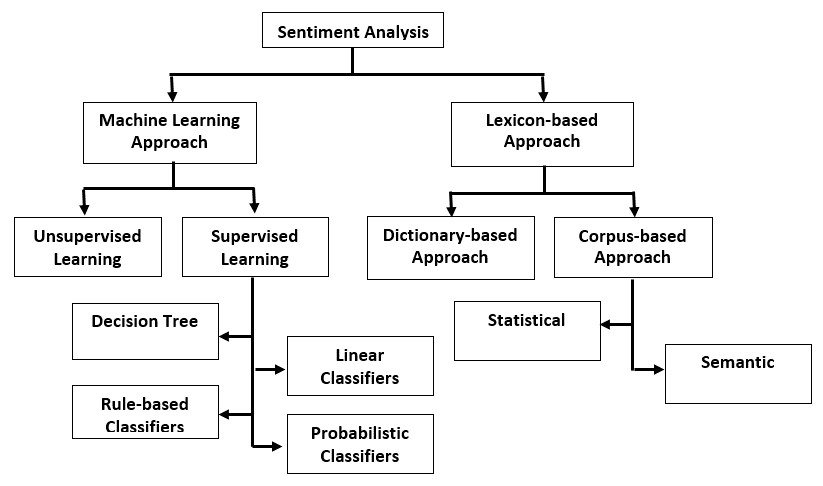
\includegraphics[scale=0.5]{images/learning_approaches_sentiment_analysis}
      \caption[Learning approaches for sentiment analysis]{Learning approaches for sentiment analysis \autocite{Halibas2018}\protect\footnotemark}
      \label{fig:learning_approaches_sentiment_analysis}
    \end{figure}
    
    \footnotetext{\url{https://www.researchgate.net/figure/Sentiment-Analysis-Source-4-Fig-1_fig1_324360275}, (11.04.2019, 23:43)}
    
    Machine learning approaches use mathematical models built by an artificial intelligence to solve the task given to them. They are split into unsupervised and supervised learning. In unsupervised learning no label of a class is provided, so there is no possibility to compare the calculated solution with the correct one. In this case a common learning approach is clustering. The input data is segmented into a (fixed) number of groups, where instances within a group should have similarities and thus form a category. In contrast, there are procedures that are to determine an output value for a given input. These are in the area of supervised learning. While regression methods can handle the assignment of continuous values, classification methods can only be applied if there is a limited and fixed number of possible output values, known as classes. \\\\
    We already defined the domain and codomain of a classification function: $\gamma:\mathbb{X}\rightarrow\mathbb{C}$. Irrespective of the choice of classification algorithm, it is recommended to split the evaluation of the procedure into a training set and a test set. Based on the training set, a model can be created that learns the characteristics of a class. Partly the training set is further subdivided, whereby a model is created on the first part of the training set and fine-tuning is performed by the second part of the set (validation set). During the evaluation the correct classes of the test instances are removed. Without prior viewing, now new classes are assigned to these instances by the learned model, which are then compared with the correct classes. If, as in the case described, only one class is assigned to each instance, it is the hard version of classifying. On the contrary, the soft version assigns to an instance a probabilistic value for each class \autocite{Aggarwal2012}. In the following some such classification learning approaches are introduced, which can be used in the area of text mining:
    \begin{itemize}
      \item Decision Trees
      
        Decision trees are designed with the use of a hierarchical division of the underlying data space with the use of different (text) features. From top to bottom, the partitions become more and more homogeneous by selection of one or several appropriate features for the decision which can be determined by measurement like information gain or Gini coefficient. This procedure can be continued until all leaves are partitions containing only one class. To avoid overfitting and reduce complexity, scarcely informative sections of the tree can be cut by pruning. Finally, a test instance is associated to the class of the partition the decision path starting from the root leads to.
      \item Pattern- or Rule-based Classifiers
      
        Rule-based classifiers are similar to decision trees; more precisely, decision trees can be represented as a set of rules. For each rule the left-hand side is a condition on the underlying feature set (usually expressed in Disjunctive Normal Form (DNF)), and the right-hand side is the class label. A rule should have a high support (absolute number of instances affected by the condition) as well as a high confidence (probability for class if condition is given). In text mining, the rule is typically expressed as a conjunction of terms that have to appear in the instance. The absence of terms is rarely used, because such rules are not likely to be very informative for sparse text data. For any test instance the class of the first rule where the condition is fulfilled will be assigned. That is why the last rule should cover all remaining instances and provide a default class.
      \item Probabilistic Classifiers
      
        Probabilistic classifiers like Bayesian classifiers calculate for each class a probability, whereby the class with the highest value is chosen for the test instance. Naïve Bayes classifiers use therefore the product of all conditional probabilities, e.g. term occurrences in different classes of texts. In comparison to other classifiers, Naïve Bayes classifiers are highly scalable because of its linear complexity. Suitable probabilistic classifiers for text mining are the Bernoulli variate model and multinomial distributions.
      \item SVM Classifiers
      
        Support-vector machines (SVM) are a subgroup of linear classifiers. A linear classifier calculates for a binary classification problem a linear predictor $p=\bar{A}\cdot\bar{X}+b$, where $\bar{X}=(x_{1}...x_{n})$ is the feature vector, $\bar{A}=(a_{1}...a_{n})$ is a vector of linear coefficients with the same dimensionality as the feature space. A natural interpretation of the linear predictor in the discrete scenario would be as a separating hyperplane between the different classes. The hyperplane with the maximum distance value to any instance, i.e. the one with the maximum margin of separation, is chosen. The SVM approach is quite robust to high dimensionality and ideally suited for text data because of the sparse high-dimensional nature of text \autocite{Joachims1997}.
      \item Neural Network Classifiers
      
        Simple neural networks are also a form of linear classifiers, since the function computed by a set of neurons is essentially linear. The simplest form of neural network, known as the perceptron (or single layer network) are essentially designed for linear separation, and work well for text. However, by using multiple layers of neurons, it is also possible to generalize the approach for non-linear separation. In such a network, the outputs of the neurons in the earlier layers feed into the neurons in the later layers. The training process of such networks is more complex, as the errors need to be back-propagated over different layers.
      \item Proximity-based Classifiers
      
        Those classifiers use proximity measures for classification. All training instances are placed in a (high-dimensional) space, proximities of two documents can be calculated by Euclidian, Manhattan or other distance measurements. Then, the most common $k$-nearest-neighbor classifier identifies for a given test instance the $k$ training instances with the smallest distance values. The most common (or highest-weighted) class among them becomes the class of the test instance.
    \end{itemize}
    In the simplest version all of the six classifier types are applied to binary classification problems. If there are three or more classes, the classifier possibly has to be extended to handle this multiclass problem, e.g. for SVM Classifiers. Another possibility is to split the multiclass problem into several binary problems as seen in subsection~\ref{subsec:multiclass_classification}. The classification is made by several classifiers that are trained to differentiate either between one class and the rest (one-against-all) or pairwise between each two classes (one-against-one). Further concepts for the customization of classifiers are boosting and bagging, the formation of ensembles or the handling of ordinal classes \autocite{Aggarwal2012}. \\\\
    For sentiment analysis problems, apart from machine learning approaches also lexicon-based approaches are suitable. Lexicon-based approaches mainly rely on a sentiment lexicon, i.e., a collection of known and precompiled sentiment terms, phrases and even idioms, developed for traditional genres of communication. To determine the polarity score of a text, the polarity scores of the terms are combined in a certain way, e.g. by addition. There are two subtypes of lexicon-based approaches. The dictionary-based approach uses a list of terms called dictionary, where the collection and scores are both created manually. Manual creation may be time-consuming, but it is usually possible to create optimally customized dictionaries with good results. The corpus-based approach uses already existent dictionaries of a specific domain, which have been constructed based on a big corpus. There are statistic techniques like latent semantic analysis (LSA) as well as semantic techniques using synonyms, antonyms or other relationships from thesaurus like WordNet \autocite{Kharde2016}.

  \subsection{Validation and evaluation}
  \label{subsec:validation_and_evaluation}
    The final step deals with the validation and evaluation of the results obtained from the previous analysis step. In subsection~\ref{subsec:definition_of_the_problem_and_goals} some performance measurements already have been presented. In the following only measurements for classification problems are discussed. Before discussing about those measurements, first of all we will specify how to arrange the data meaningfully to be able to perform most of the measurements. \\\\
    We already mentioned that for the evaluation the data should be split into a training and a test set. Formally speaking, a training set $\mathbb{D}$ of labeled documents $\langle d,c\rangle$ is given, where $\langle d,c\rangle\in\mathbb{X}\times\mathbb{C}$. For all unlabeled documents $d$ in the test set, the chosen classification function(s) $\gamma$ has to predict a class $c$ \autocite[Chapter~13.1]{Manning2008}. Generally, the larger the training set the better the classifier, although the returns begin to diminish once a certain volume of training data is exceeded. And the larger the test set, the more accurate the error estimate. There are different approaches to deal with this problem \autocite[Chapter~5]{Witten2005}:
    \begin{itemize}
      \item Holdout method
      
        The simplest approach is to determine a specific percentage that should be used for training (usually two thirds). The rest of the data is cut and hold out for the final validation of unseen data. Note that here data can either be used for training or for testing.
      \item k-fold-Cross-validation
      
        The cross-validation tries to get away from wasting data by using all data both for training and for testing in different iterations. The data is split into $k$ folds (usually 10); $k-1$ of them are used for training and the remaining one for validation. The final measurement is the average of the measurement of all $k$ iterations and should outbid the simple holdout method in the performance value as well as in its accuracy. A non-random decomposition into folds, e.g. by previous sorting of the data records, can falsify the results.
      \item Leave-one-out-validation
      
        For even smaller data sets the leave-one-out-validation is a suitable approach. Here only one test instance is validated while the rest is used for training. This results in $n$ possible iterations where $n$ is the size of the data set. Similar approaches for small data sets with even more possible iterations are the leave-k-out-validation ($\binom{n}{k}$ possiblities) and the bootstrap method \autocite[Chapter~4]{Arlot2010}.
    \end{itemize}
    Of course, it could be also possible not to distinguish between training and test data, i.e. the model is built and evaluated based on all data. However, this approach can lead to overfitted and therefore overestimated performance values that generally cannot be sustained in real application cases when predictions have to be made for unseen data. \\\\
    The accuracy has already been presented as a simple yet meaningful measurement value. Before it is calculated, a confusion matrix $M$ is usually created, where a value $M_{ij}$ specifies how many instances of the class $i$ were classified as class $j$. The accuracy is the sum of all values in the main diagonal of the confusion matrix (i.e. $i=j$) divided by the total number of instances. \\\\
Instead of using an absolute accuracy value it can make sense to use a relative one. In classification problems a baseline can be used as a comparison value for the accuracy. \citeauthor{Witten2005} use an expected value calculated by a default classifier as shown on the right side of table~\ref{tab:actual_and_expected_outcomes_of_three_class_classification}. They assume that the comparison classifier predicts each individual class with the same frequency as the original one. This classifier predicts for $60+18+4=82$ instances the correct class (right side), while the original does for $88+40+12=140$ (left side). This results in $140-82=58$ additional correct classifications out of $200-82=118$ and a kappa statistic of $58\div118=49.2\%$. Another meaningful value to compare is the baseline accuracy, which is achieved by a classifier always selecting the most frequently occurring class. In the example above the baseline classifier achieves $100$ correct classification which would decrease the kappa statistic to $40\%$. Obviously, a kappa statistic of $100\%$ would indicate a perfect classifier, a value of $0\%$ no improvement and a negative value even a deterioration.
  
    \begin{table}[H]
      \begin{tabular}{cc|c|c|c|c|l}
        \cline{3-5}
        & & \multicolumn{3}{ c| }{Predicted class} \\ \cline{3-6}
        & & a & b & c & Total \\ \cline{1-6}
        \multicolumn{1}{ |c  }{\multirow{3}{*}{Actual class} } &
        \multicolumn{1}{ |c| }{a} & 88 & 10 & 2 & 100 & \\ \cline{2-6}
        \multicolumn{1}{ |c  }{} &
        \multicolumn{1}{ |c| }{b} & 14 & 40 & 6 & 60 & \\ \cline{2-6}
        \multicolumn{1}{ |c  }{} &
        \multicolumn{1}{ |c| }{c} & 18 & 10 & 12 & 40 & \\ \cline{1-6}
        \multicolumn{1}{  c  }{} &
        \multicolumn{1}{ |c| }{Total} & 120 & 60 & 20 & 200 & \\ \cline{2-6}
      \end{tabular}      
      \begin{tabular}{cc|c|c|c|c|l}
        \cline{3-5}
        & & \multicolumn{3}{ c| }{Predicted class} \\ \cline{3-6}
        & & a & b & c & Total \\ \cline{1-6}
        \multicolumn{1}{ |c  }{\multirow{3}{*}{Actual class} } &
        \multicolumn{1}{ |c| }{a} & 60 & 30 & 10 & 100 & \\ \cline{2-6}
        \multicolumn{1}{ |c  }{} &
        \multicolumn{1}{ |c| }{b} & 36 & 18 & 6 & 60 & \\ \cline{2-6}
        \multicolumn{1}{ |c  }{} &
        \multicolumn{1}{ |c| }{c} & 24 & 12 & 4 & 40 & \\ \cline{1-6}
        \multicolumn{1}{  c  }{} &
        \multicolumn{1}{ |c| }{Total} & 120 & 60 & 20 & 200 & \\ \cline{2-6}
      \end{tabular}      
      \caption[Outcomes of three-class-classification]{Actual (left) and expected (right) outcomes of three-class-classification, cf.\autocite[Chapter~5.7]{Witten2005}}
      \label{tab:actual_and_expected_outcomes_of_three_class_classification}
    \end{table}
      
    In the kappa statistics just presented it is assumed that all false classifications are equally weighted. However, there are also cases where a classifier with negative kappa statistics is preferable to a baseline classifier. Medical classifications of patients into the classes healthy and sick are a prime example of this. A classifier with $98\%$ accuracy caused by $2\%$ of false positives (healthy patients misclassified as sick) is usually preferable to the baseline classifier with $99\%$ accuracy and the only output healthy and therefore $1\%$ of false negatives (sick patients misclassified as healthy). This is because in this case false negatives weigh heavier than false positives. For this reason, in cost-sensitive classification problems the exact cost factors for each cell in the confusion matrix have to be defined before determining a baseline classifier and an appropriate kappa statistic. In ordinal classification problems the baseline classifier with minimal costs might have the average class as the only output instead of the most common class. The influence of costs in cost-sensitive learning have already been discussed in subsection~\ref{subsec:cost_sensitive_learning}. \\\\
    Apart from the accuracy there are further measurement values like recall and precision. Given the confusion matrix $M$, precision and recall are defined as
    \[precision_{i}=\frac{M_{i i}}{\sum_{j}M_{ji}} \quad \textrm{and} \quad recall_{i}=\frac{M_{i i}}{\sum_{j}M_{ij}}\]
    The precision thus describes how high the quota of correctly classified instances is among all instances classified as class $i$, while the recall describes the quota of correctly classified instances among all instances that actually belong to class $i$. In binary classification problems, the formulas are simplified into
    \[precision=\frac{tp}{tp+fp} \quad \textrm{and} \quad recall=\frac{tp}{tp+fn}\]
    where $tp$ is true positives, $fp$ false positives and $fn$ false negatives. Precision and recall generally have a negative correlation and cannot be optimized at the same time. As a compromise the F-measure can be used which forms the harmonic mean of precision and recall:
    \[F=2\cdot\frac{\text{precision}\cdot\text{recall}}{\text{precision}+\text{recall}}\]
    The Receiver Operating Characteristic (ROC) is an alternative to the precision and recall measurement which visualizes the ratio of true and false positives. The confusion matrix provides only one single point for a classifier, which is generally the better the closer it is to the optimal point (0|1) indicating $0\%$ false positives (and therefore $100\%$ true negatives and optimal precision) and $100\%$ true positives (and therefore $0\%$ false negatives and optimal recall). Because false positives and false negatives can be weighted differently, the Euclidian distance has to be adjusted by different weights for the $x$- and $y$-direction. If the output values of a classifier are ranked (e.g. by probability or relevance), a whole ROC curve can be created
    \begin{itemize}[noitemsep]
      \item starting at the point (0|0),
      \item moving $\frac{1}{P}$ units to the top in case of a true positive (where $P$ is the total number of positives),
      \item moving $\frac{1}{N}$ units to the right in case of a false positive (where $N$ is the total number of negatives)
      \item and ending at the point (1|1).
    \end{itemize}
    In this case, the Area Under ROC Curve (AUC) is another possible indicator for a good classification. It also has a nice interpretation as the probability that the classifier ranks a randomly chosen positive instance above a randomly chosen negative one. Although those definitions and interpretations only work for binary classification problems, there are customized variants for multiclass classification, see \autocite{Hand2001}.

  \clearpage
  
  \section{Experimental setup}
  \label{sec:experimental_setup}
  
  \subsection{Data set extraction}
    Nur Weka-Classification oder auch ersten Ansatz der NLTK-Classification mit reinnehmen?

  \subsubsection{PGN-format}
    PGN is "Portable Game Notation", a standard designed for the representation of chess game data using ASCII text files. PGN is structured for easy reading and writing by human users and for easy parsing and generation by computer programs \autocite[Chapter~1]{Edwards1994}. A sample game in PGN notation is shown in figure~\ref{fig:sample_pgn_game}.

	\begin{figure}[H]
	  \centering
      \lstset{commentstyle=\color{blue},morecomment=[s]{\{}{\}},moredelim=[is][\bfseries]{\\textbf\{}{\}},moredelim=[is][\color{red}]{\\nag\{}{\}}}
	  \begin{lstlisting}	  
[Event "Deutschland "]
[Site "?"]
[Date "1995.??.??"]
[Round "?"]
[White "Lutz, Ch"]
[Black "Kramnik, V."]
[Result "0-1"]
[ECO "B33"]
[PlyCount "70"]
[EventDate "1995.??.??"]

\textbf{1. e4} {B33: Sicilian: Pelikan and Sveshnikov Variations} \textbf{1... c5 2. Nf3 Nc6 3.
d4 cxd4 4. Nxd4 Nf6 5. Nc3 e5 6. Ndb5 d6 7. Bg5 a6 8. Na3 b5 9. Nd5 Be7 10.
Bxf6 Bxf6 11. c3 O-O 12. Nc2 Bg5 13. a4 bxa4 14. Rxa4 a5 15. Bc4 Rb8 16. b3 Kh8
17. O-O g6 18. Qe2 Bd7 19. Rfa1 19... Bh6} {last book move} \textbf{20. g3} {
Consolidates f4} (20. Nde3 20... Be6 \nag{$14}) \textbf{20... f5} \nag{$11} \textbf{21. exf5 gxf5 22. b4
22... e4} {Black wins space.} \textbf{23. bxa5 Ne5 24. Rb4 Rxb4 25. cxb4 f4 26. Nd4 e3
27. fxe3} (27. Nxf4 \nag{$2} {doesn't work because of} 27... exf2+ 28. Qxf2 28... Bxf4
\nag{$19}) \textbf{27... f3} {He broke from his leash} (27... fxg3 28. hxg3 Qg5 29. Kh2 Nxc4
30. Nf4 \nag{$19}) \textbf{28. Qa2 f2+ 29. Kg2 Qe8 30. Be2 30... Ng4} {
The pressure on the isolated pawn grows} \textbf{31. Bf3} \nag{$4} (31. Qd2 Qh5 32. Bxg4 Qxg4
33. Nf4 Bxf4 34. exf4 Qh3+ 35. Kxf2 Qxh2+ 36. Ke1 Qxg3+ 37. Kd1 Qg1+ 38. Ke2
Bg4+ 39. Kd3 Qxa1 40. f5 \nag{$19}) \textbf{31... Nxe3+} \nag{$19} \textbf{32. Nxe3 Qxe3 33. Qxf2} \nag{$4} {
sad, but how else could White save the game?.} (33. Rd1 Bg7 34. Qb3 Bxd4 35.
Qxe3 Bxe3 36. Be2 \nag{$19}) \textbf{33... Bh3+} \nag{$1} {the final blow} \textbf{34. Kg1} {
Black now must not overlook the idea Re1} (34. Kxh3 {A deflection} 34... Qxf2)
\textbf{34... Qc3 35. Re1 Bd2} (35... Bd2 36. Ne2 36... Qxf3 \nag{$19} (36... Bxe1 \nag{$6} {
is clearly weaker} 37. Nxc3 Bxf2+ 38. Kxf2 \nag{$19}) (36... Rxf3 \nag{$2} 37. Nxc3 Rxf2
38. Kxf2 Bxc3 39. Re7 \nag{$18})) \textbf{0-1}
	  \end{lstlisting}	  

      \caption{Sample PGN game}
      \begin{tabular}{r@{: }l r@{: }l}
        blue & comments & red & NAGs
      \end{tabular}
      \label{fig:sample_pgn_game}
	\end{figure}
	
    A PGN game contains first a list of tuples with general information of the game (“tag pairs”). Seven of those tags are mandatory (Seven Tag Roster: Event, Site, Date, Round, White, Black, Result), the other tags are optional. \\\\
    Afterwards the “movetext” section starts. The chess moves themselves are represented using SAN (Standard Algebraic Notation). A move pair (one move of white and one of black) starts with the move pair number followed by a dot and a blank, then the move of white, another blank and the move of black, e.g. 
    \begin{quotation}
      7. Bg5 a6.
    \end{quotation}    
    Each move contains the piece by a single upper-case letter except of the pawn (see table~\ref{tab:basic_chess_notations}) followed by the square the piece is moved to (see figure~\ref{fig:square_names}). Hence, the example describes the seventh move of both players in the game; white moves his dark-squared bishop to the square g5 and black moves his a-file-pawn to a6. If a piece of the opponent is placed on the destination square, this piece is captured and in the move an "x" is inserted immediately before the destination square. In this case, if the capturing piece is a pawn, the lower-case letter of the previous file of the pawn is used at the beginning of the move, e.g. "exd5". Whenever a move pair is interrupted by a comment, the move of black is prefaced by the move pair number, an ellipsis and a blank: 
    \begin{quotation}
      Nxf4 \$2 \{doesn't work because of\} 27... exf2+
    \end{quotation}
    Additionally, there are some further moves with a special notation (see table~\ref{tab:basic_chess_notations}). In cases of disambiguation of pieces, an additional letter for the file or a number for the rank is used. In summary, a move can contain between two and seven signs in SAN \autocite[Chapter~8]{Edwards1994}.
	
    \begin{figure}[H]
      \begin{floatrow}
      \capbtabbox[10.4cm]{%
        \begin{tabular}{| l | l |}
    	\hline
    	Symbol & Meaning \\ \hline
    	  K & King \\ \hline
    	  Q & Queen \\ \hline
    	  R & Rook \\ \hline
    	  B & Bishop \\ \hline
    	  N & Knight \\ \hline
    	  \textit{blank} & Pawn \\ \hline
        \end{tabular}
        \begin{tabular}{| l | l | l |}
    	  \hline
    	  Symbol & Meaning & Example \\ \hline
    	  x & Capture & Rxa1 \\ \hline
    	  + & Check & Nf6+ \\ \hline
    	  \# & Checkmate & Bb7\# \\ \hline
    	  0-0 & Castling kingside & \\ \hline
    	  0-0-0 & Castling queenside & \\ \hline
    	  = & Promotion & fxg1=Q+ \\ \hline
        \end{tabular}
      }{%
        \caption{Basic chess notations}
        \label{tab:basic_chess_notations}
      }
      \ffigbox[6.6cm]{%
	    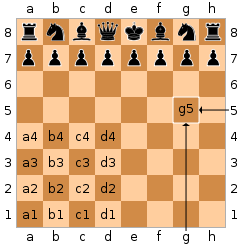
\includegraphics[scale=0.5]{images/algebraic_notation}
      }{%
	    \caption[Square names in algebraic notation]{Square names in algebraic notation\protect\footnotemark}
        \label{fig:square_names}
      }
      \end{floatrow}
    \end{figure}
    
  	\footnotetext{\url{https://en.wikipedia.org/wiki/Algebraic_notation_(chess)#/media/File:SCD_algebraic_notation.svg}, (18.03.2019, 20:56)}
  	
	Parts of the moves are annotated using comments in braces. A comment can contain information about the opening of the game, about a single move or about the current position. In the last two cases the comment is often prefaced by one or several NAGs (see below) or the corresponding chess symbol. Since there is no restriction on the exact position of a comment, comments may refer to the move before or after itself. A comment can also connect two or more moves with each other. On the contrary, a comment can be interrupted by a move such that it is split into two parts, which may only make sense when seen together. All in all, there are four possibilities of comment-move combinations shown in the examples of table~\ref{tab:comment_move_combinations}.
	
	\begin{table}[H]
      \centering
      \begin{tabular}{| l | l |}
    	\hline
    	Combination & Example \\ \hline
    	Move, Comment & e4 \{Black wins space.\} \\ \hline
    	Comment, Move & \{Weaker is\} 39. Bxe6 \\ \hline
    	Move, Comment, Move & Nxf4 \$2 \{doesn't work because of\} 27... exf2+ \\ \hline
    	Comment, Move, Comment & \{Because of the blunder\} 24. Txf8 \{Black wins immediately\} \\ \hline
      \end{tabular}      
      \caption{Comment-move combinations}
      \label{tab:comment_move_combinations}
    \end{table}
    
    Besides, by convention there should not be nested braces, however, sometimes nested braces are used to comment different move variants separately.	Those variants need not be part of a comment and are written down in parenthesis. The enumeration of the moves proceeds within a variant and is set back before a new variant starts or the game itself continues. 
   
  \subsubsection{Chessbase-DB}
  	Transformation to PGN, language detection using polyglot
  
  \subsubsection{NAGs}
	Symbols and corresponding NAGs
	
	\begin{table}[H]
      \begin{tabular}{| l | l | l |}
    	\hline
    	NAG & Symbol & Meaning \\ \hline
    	x & Capture & Rxa1 \\ \hline
    	+ & Check & Nf6+ \\ \hline
    	\# & Checkmate & Bb7\# \\ \hline
    	0-0 & Castling kingside & \\ \hline
    	0-0-0 & Castling queenside & \\ \hline
    	= & Promotion & fxg1=Q+ \\ \hline
      \end{tabular}
      \caption{Meaning of NAGs}
      \label{tab:meaning_of_nags}
	\end{table}

  \subsubsection{Python NLTK}
	RegExp parsing, tokenization, extraction of comment and class  
  
  \subsection{Prepare data for classification}

  \subsubsection{Feature extraction}
    simple features: count(word), advanced features: tf-idf, bigrams, trigrams

  \subsubsection{Generating training instances}
    structure of arff-file
	a brilliant counterattack of white
	a big mistake of black	   
    
    \newsavebox{\complete}
      \begin{lrbox}{\complete}
        \lstset{keywordstyle=\color{blue},morekeywords={@RELATION,@ATTRIBUTE,@DATA,NUMERIC,REAL}}
        \begin{lstlisting}
@RELATION comment
@ATTRIBUTE COUNT(brilliant) NUMERIC
@ATTRIBUTE TFIDF(mistake) REAL
@ATTRIBUTE CLASS {good,bad}
@DATA
1, 0.0, good
0, 0.06, bad	  
        \end{lstlisting}
      \end{lrbox}
    \newsavebox{\sparse}
      \begin{lrbox}{\sparse}
        \lstset{keywordstyle=\color{blue},morekeywords={@RELATION,@ATTRIBUTE,@DATA,NUMERIC,REAL}}
        \begin{lstlisting}
@RELATION comment
@ATTRIBUTE COUNT(brilliant) NUMERIC
@ATTRIBUTE TFIDF(mistake) REAL
@ATTRIBUTE CLASS {good,bad}
@DATA
{1 2, 3 good}
{2 0.06, 3 bad}	  
        \end{lstlisting}
      \end{lrbox}    
    
    \begin{figure}[H]
	  \centering      
	  \subfloat[complete]{\usebox{\complete}}
	  \quad
	  \subfloat[sparse]{\usebox{\sparse}}
      \caption{Sample arff files}
      \label{fig:sample_arff_files}
	\end{figure}
  \clearpage
  
  \section{Experiment setup}
  
  \subsection{Selecting classes}
    distribution how many instances per class, splitting into several problems: 2 classes (!,?), 6 classes (!!,!,!?,?!,?,??), 2 classes (+,-), 7 classes --> introduction of dictionary
    difference if even or odd number of classes ("neutral class")
    
  \subsection{Tokenizer tuning}
    punctuation, special chess notations (\#ce etc.)
    
  \subsection{NLTK Parameters}
    stopwords, stemming, threshold(hapax), lowercase, bigram, trigram

  \subsection{Classifiers}
    which classifier to use? --> MCC (x3), OCC, RF, NBM
  \clearpage  
  
  \section{Evaluation of results}
    tables with number of attributes, tables with accuracies, comparison of confusion matrix\\
    each for simple approach, tf-idf, word embedding
  \clearpage  
  
  \section{Conclusion}

  \subsection{Summary}

  \subsection{Outlook}
  \clearpage
  
  \paragraph{References}
  \printbibliography
  \clearpage
  
\end{document}
